\documentclass{rtxreport}

\author{Thomas Luquet}

\title{Bilan Architecture}

\rtxdoctype{Bilan Architecture}
\rtxdocref{2012\_AA1\_FR\_Rathaxes}
\rtxdocversion{0.8}
\rtxdocstatus{Finale}

\rtxdochistory{
0.1 & 16/11/2010 & Thomas Luquet & Premier draft \\
\hline
0.2 & 17/11/2010 & Louis Opter & Fix compilation \\
\hline
0.3 & 17/11/2010 & Louis Opter & Ajout du cartouche \\
\hline
0.4 & 17/11/2010 & David Pineau & Completion de la section Technologie \\
\hline
0.5 & 17/11/2010 & Louis Opter & Reformulations et ajout de notes \\
\hline
0.6 & 17/11/2010 & Thomas Luquet & Reformulation, inssertion de graphique \\
\hline
0.7 & 17/11/2010 & Luquet Thomas & Reformulation, corrections diverses \\
\hline
0.8 & 17/11/2010 & Louis Opter & Relecture et corrections \\
}

\newcommand{\note}[1]{\marginpar{\scriptsize{\textdagger\ #1}}}

\begin{document}

\maketitle

\rtxmaketitleblock

\tableofcontents

\chapter{Rappel du projet}

\section{Qu'est ce que \rtx\ ?}

\rtx\ est un ensemble d'outils permettant de simplifier l'écriture de pilote de
périphérique. Le projet permet de générer un code source écrit en C pour Linux,
Windows 7 et OpenBSD à partir d'un fichier de description de pilote.

C'est un projet à visée scientifique distribué sous licences libres.

Le projet \rtx\ 2012 est une amélioration de l'EIP réalisé en 2009. Il
incorpore de nouvelles fonctionnalitées comme l’asynchronicité. \rtx\ 2012 sera
capable de générer un pilote de souris USB et celui d'une carte son qui
serviront à prouver que le concept fonctionne.

\section{Structure du projet}

% Ne pas dire Rathaxes ici car juste en dessous on dit que c'est un
% compilateur…
Le projet est divisé en trois parties :
\begin{enumerate}
\item Le langage \rtx\ : un langage dédié (DSL\footnote{Domain Specific
Language.}) utilisé pour décrire un pilote~;
\item La black-librarie : Elle permet l'interfaçage entre le DSL et le
compilateur~;
\item Le compilateur : Il transforme les fichiers \rtx\ (.rtx) ---à l'aide
de la black-librairie--- en fichier .c spécifiques au système d'exploitation choisi.
\end{enumerate}

\chapter{Diagrammes}

\section{Description fonctionelle}

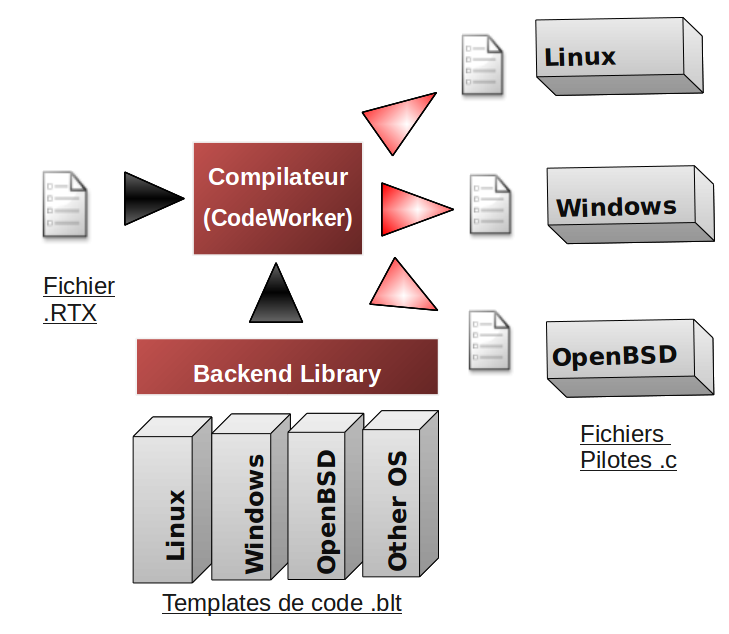
\includegraphics[width=\textwidth]{diagramme_general}

\rtx\ est un compilateur.

Il utilise le langage CodeWorker pour l'analyse du DSL ainsi que la génération
d'un AST\footnote{Abstract Syntax Tree, Arbre de Syntaxe Abstraite.}. Enfin,
CodeWorker utilise cet AST, pour générer le code C du driver. Afin de pouvoir
générer du code C à partir du DSL de \rtx\, le compilateur utilise une
bibliothèque de modele appelé Backend Library. % Qui génére quoi ?

\section{Diagramme détaillé}

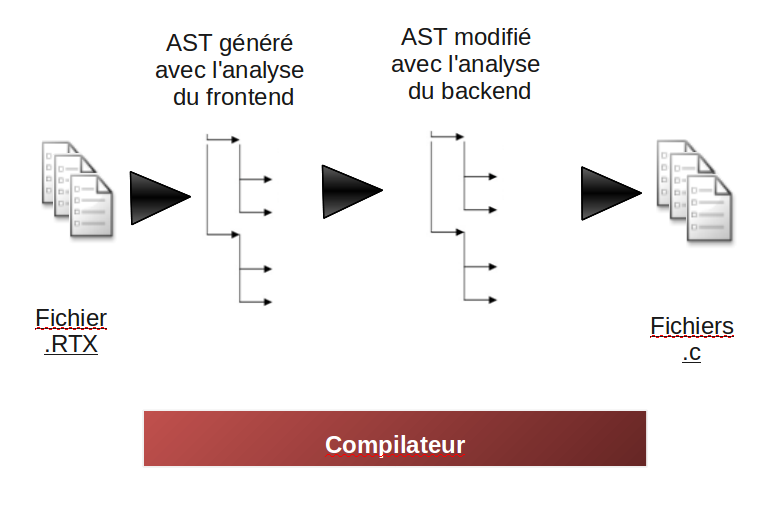
\includegraphics[width=\textwidth]{diagramme_fonctionel}

Actuellement le compilateur \rtx\ de la promotion 2009 fonctionne ainsi~:
\begin{enumerate}
\item Il transforme les fichier \texttt{.rtx} (écrit dans le DSL \rtx) en un AST ;
\item Il parcourt cet arbre. En fonction des mots clefs rencontrés, le
compilateur selectionne des fichiers BLT issus de la backend Library ; % D'où sorte les mots BLT et "backend library" ?
\item Enfin il génère des fichiers de pilote de périphérique selon l'arbre
reconstruit à partir des modèles de la BLT.
\end{enumerate}

Notre objectif est de modifier le comportement du compilateur dans le but
rendre les modifications futur du langage plus simple à implémenter.

Pour cela l'étape de transformation de l'AST en fichier \texttt{.c} sera
segmentée en 2 étapes :
\begin{enumerate}
% j'ai remplacé "bouts" par échantillons, la phrase est toujours
% incompréhensible mais au moins on a plus l'impression du faire du patchwork :
\item Modifier l'AST généré à partir du DSL. L'équipe insérera des échantillons
d'AST généré à partir de fichiers de la Backend Librarie activé selon les mots
clefs du DSL ;
\item Transcrire l'arbre final en langage C.
\end{enumerate}

\chapter{La technologie \rtx}

\section{Un héritage}

Un grand nombre de choix technologiques ont été effectués par l'équipe 2009.
Ils avaient besoin d'une technologie permettant d'implémenter facilement un
compilateur, qui puisse utiliser des modèles de code.

\subsection{Un compilateur}

Pour écrire le compilateur, l'outil retenu par la première équipe est
CodeWorker. CodeWorker est un langage interprété dont la syntaxe s'inspire la
notation EBNF\footnote{Extended Backus--Naur Form}. L'interpréteur CodeWorker
est distribué gratuitement sous la licence libre LGPL.

CodeWorker, présente l'avantage d'être facilement abordable et permet une
analyse syntaxique et lexicale avancée, tout en permettant la génération de
code en se basant sur l'arbre de syntaxe abstraite généré par le code
précédemment analysé.

De plus, la syntaxe proposée pour le langage de script de CodeWorker est pour
la partie analyse syntaxique relativement proche de la syntaxe EBNF. De même,
la syntaxe proposée pour le script de manipulation d'arbre syntaxique et de
génération est dérivée du C, la rendant relativement familière à l'ensemble de
l'équipe qui maitrise le C.

\subsection{Une série de modèles}

L'objectif du projet est de générer des drivers en C pour différents systèmes
d'exploitation. Ceci doit être fait en indépendance des connaissances
spécifiques à un OS. Il est donc nécessaire de posséder un système de modèles
de code utilisables pour générer du code C pour chaque système spécifique.

C'est aussi pour cela que l'équipe 2009 a choisi CodeWorker comme l'outil le plus
pratique. En effet, la solution la plus simple pour avoir des modèles de code
qui permetent de générer du code C est d'écrire directement des modèles
en script CodeWorker, de manière a réduire la quantité de travail nécessaire
du côté du backend de \rtx\ (pour la partie parsing).

\section{Un langage}

Forts de l'expérience acquise par l'équipe 2009 de \rtx, l'objectif de
notre groupe est de rechercher et implémenter de nouveaux concepts dans
\rtx. Parmi ceux-ci, s'illustre notemment les notions d'asynchronicité,
de DMA\footnote{Direct Memory Access.}, d'IRQ\footnote{Interrupt ReQuest.} et
enfin l'ensemble des concepts liés a l'utilisation de BUS tels que le PCI dans
les pilotes de périphériques.

Un autre objectif de notre équipe est d'apporter des améliorations dans le
fonctionnement même de \rtx. Jusqu'alors, le code C était généré par
activation des modèles en fonction du contenu de l'arbre de syntaxe abstraite.
Nous désirons changer cela, pour d'une part rendre le coeur du compilateur
plus générique, et permettre de tester efficacement chaque étape
d'implémentation du langage.

Pour cela, nous allons conserver le CodeWorker, qui par sa simplicité, nous
permettra de modifier le coeur du compilateur, afin par la suite de pouvoir
facilement intégrer de nouveaux concepts et mots clefs au compilateur. Par
ailleurs nous pourrons intégrer plus aisément des contributeurs externes au
projet.

\end{document}
